\documentclass{article}
%%%%%%%%%%%%%%%%%%%%%%%%%%%%%%%%%%%%%%%%%%%%%%%%%%%%%%%%%%%%%%%%%%%%%%%%%%%%%%%
% PREAMBLE
%%%%%%%%%%%%%%%%%%%%%%%%%%%%%%%%%%%%%%%%%%%%%%%%%%%%%%%%%%%%%%%%%%%%%%%%%%%%%%%
\usepackage{mathtools}
\usepackage{algorithm}
\usepackage{algorithmic}
\usepackage{fancyvrb}
\usepackage{booktabs}
\usepackage{rotating}
\usepackage{tikz}
\usepackage{float}
\usepackage{hyperref}
\usepackage{subcaption}
\usetikzlibrary{arrows,decorations.pathmorphing,backgrounds,positioning,fit,matrix}
\newcommand{\DepProps}{\textsc{DepProps}}
\usepackage{titling}
\newcommand{\subtitle}[1]{%
  \posttitle{%
    \par\end{center}
    \begin{center}\large#1\end{center}
    \vskip0.5em}%
}
\begin{document}
% TITLE
\title{DM207 I/O-Efficient Algorithms and Data Structures}
\subtitle{Fall 2015\\Project 1}
% AUTHER
\author{Mikkel Levisen and Jesper Lund}
%DATE
\maketitle
% no page number on first page
\thispagestyle{empty}
\newpage
% TABLE OF CONTENTS
\tableofcontents
% no page number on table of contents page
\thispagestyle{empty}
\newpage
% restart page number counter
\pagenumbering{arabic} 
%%%%%%%%%%%%%%%%%%%%%%%%%%%%%%%%%%%%%%%%%%%%%%%%%%%%%%%%%%%%%%%%%%%%%%%%%%%%%%%
% DOCUMENT START
%%%%%%%%%%%%%%%%%%%%%%%%%%%%%%%%%%%%%%%%%%%%%%%%%%%%%%%%%%%%%%%%%%%%%%%%%%%%%%%
\section{Introduction}
MOJN
\section{Tasks}
\subsection{1}
\begin{figure}[p]
    \centering
    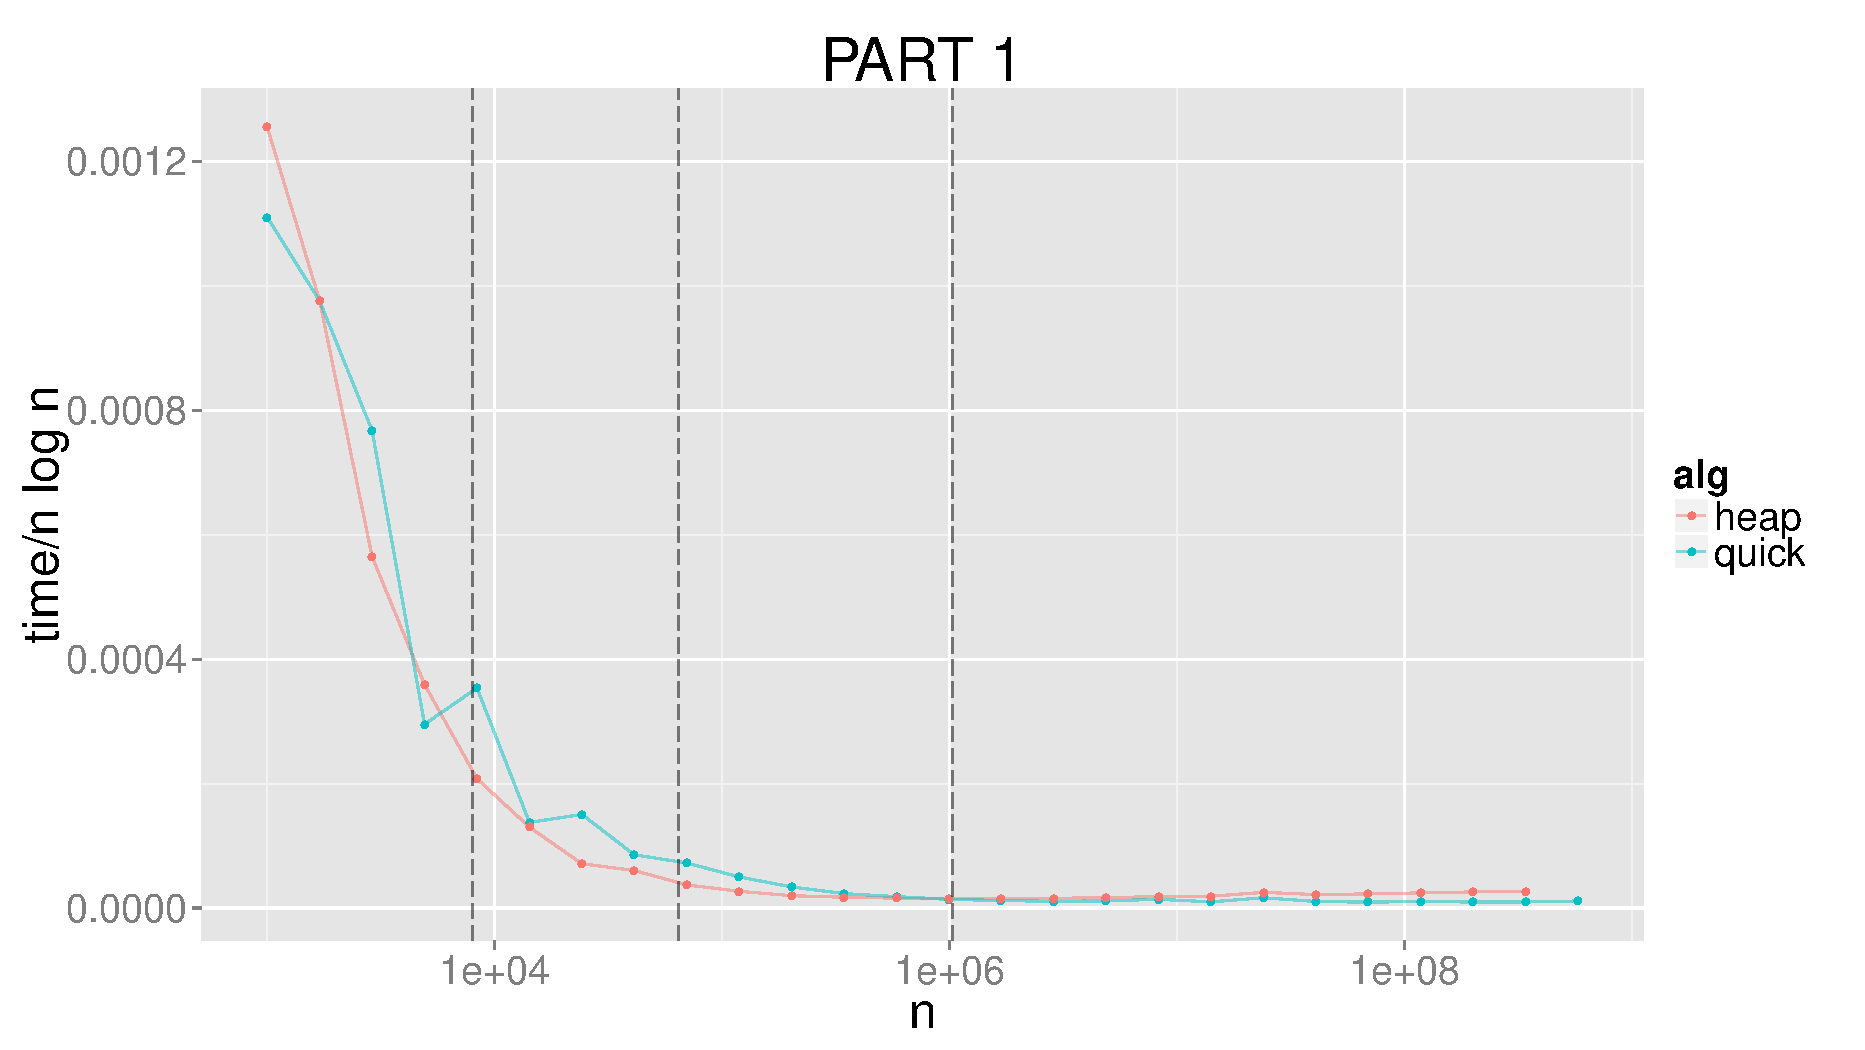
\includegraphics[width=
    \textwidth]{images/part1.pdf}
    \caption{Awesome Image}
    \label{fig:awesome_image}
\end{figure}
\subsection{2}
\begin{figure}[p]
    \centering
    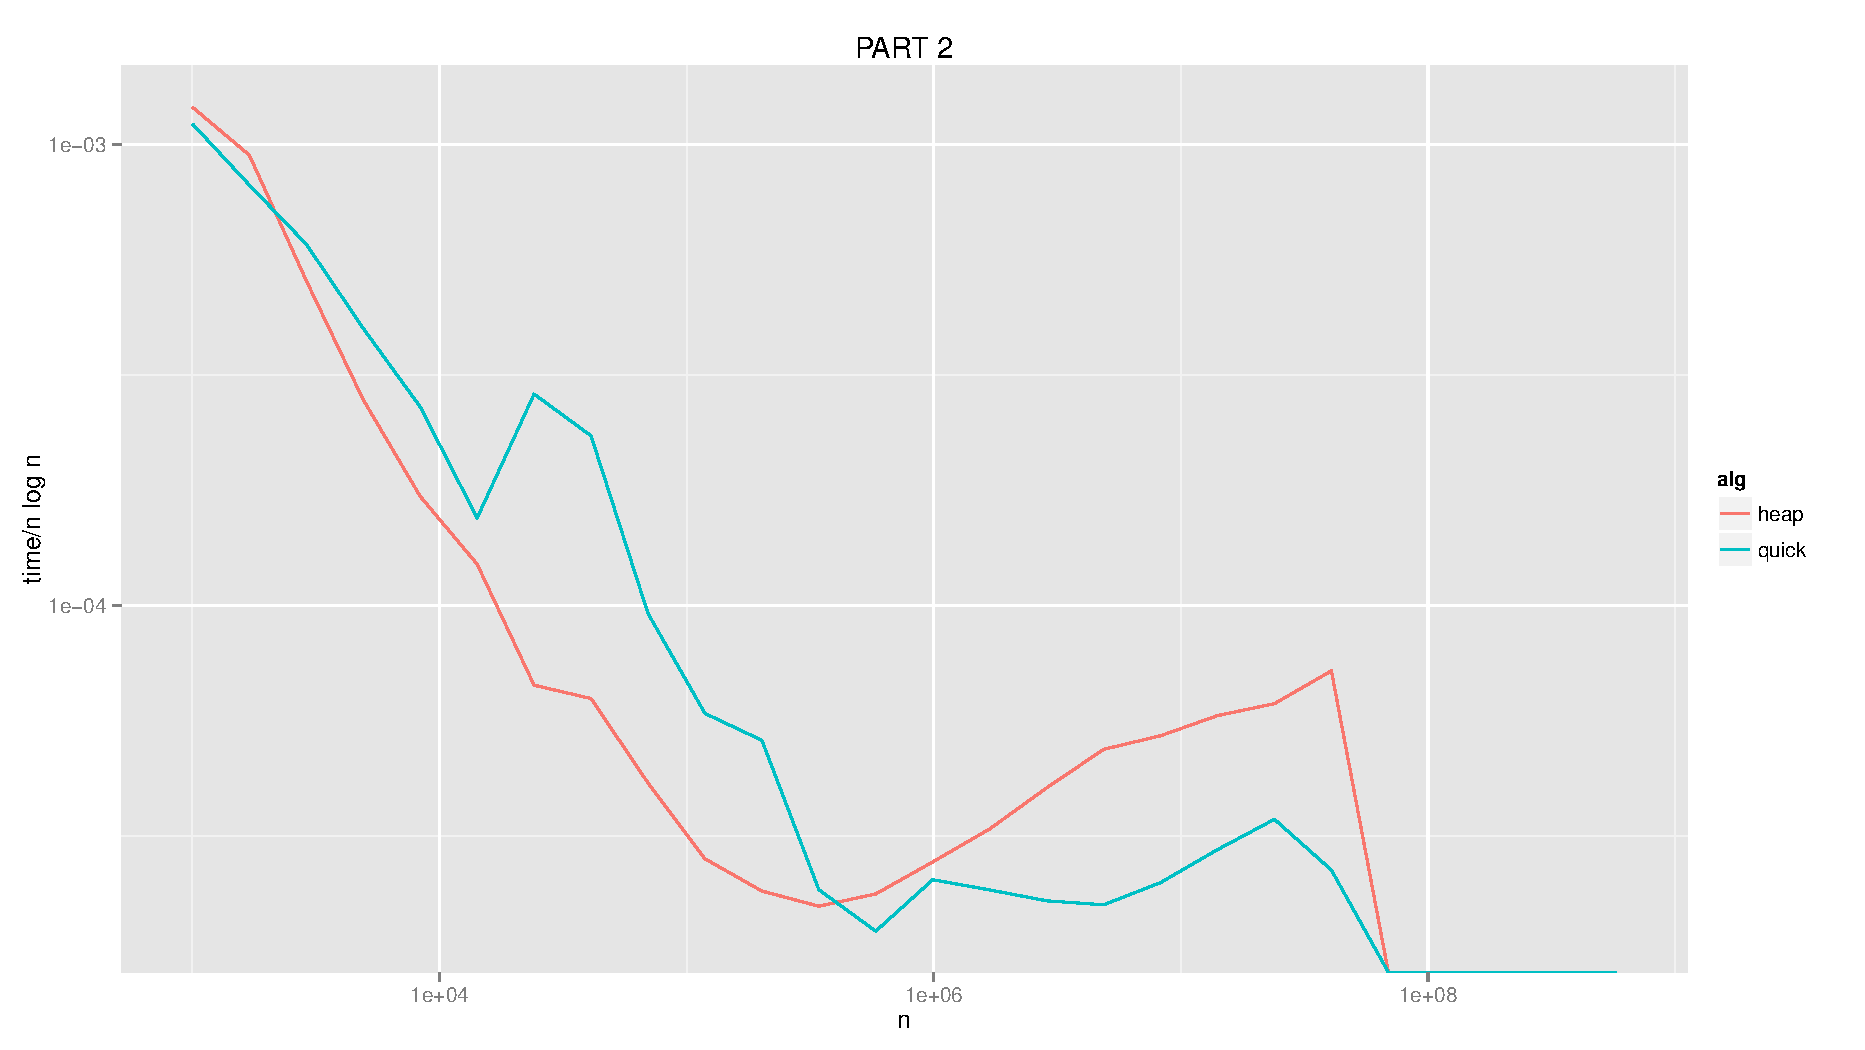
\includegraphics[width=
    \textwidth]{images/part2.pdf}
    \caption{Awesome Image}
    \label{fig:awesome_image}
\end{figure}
\subsection{3}
\begin{figure}[p]
    \centering
    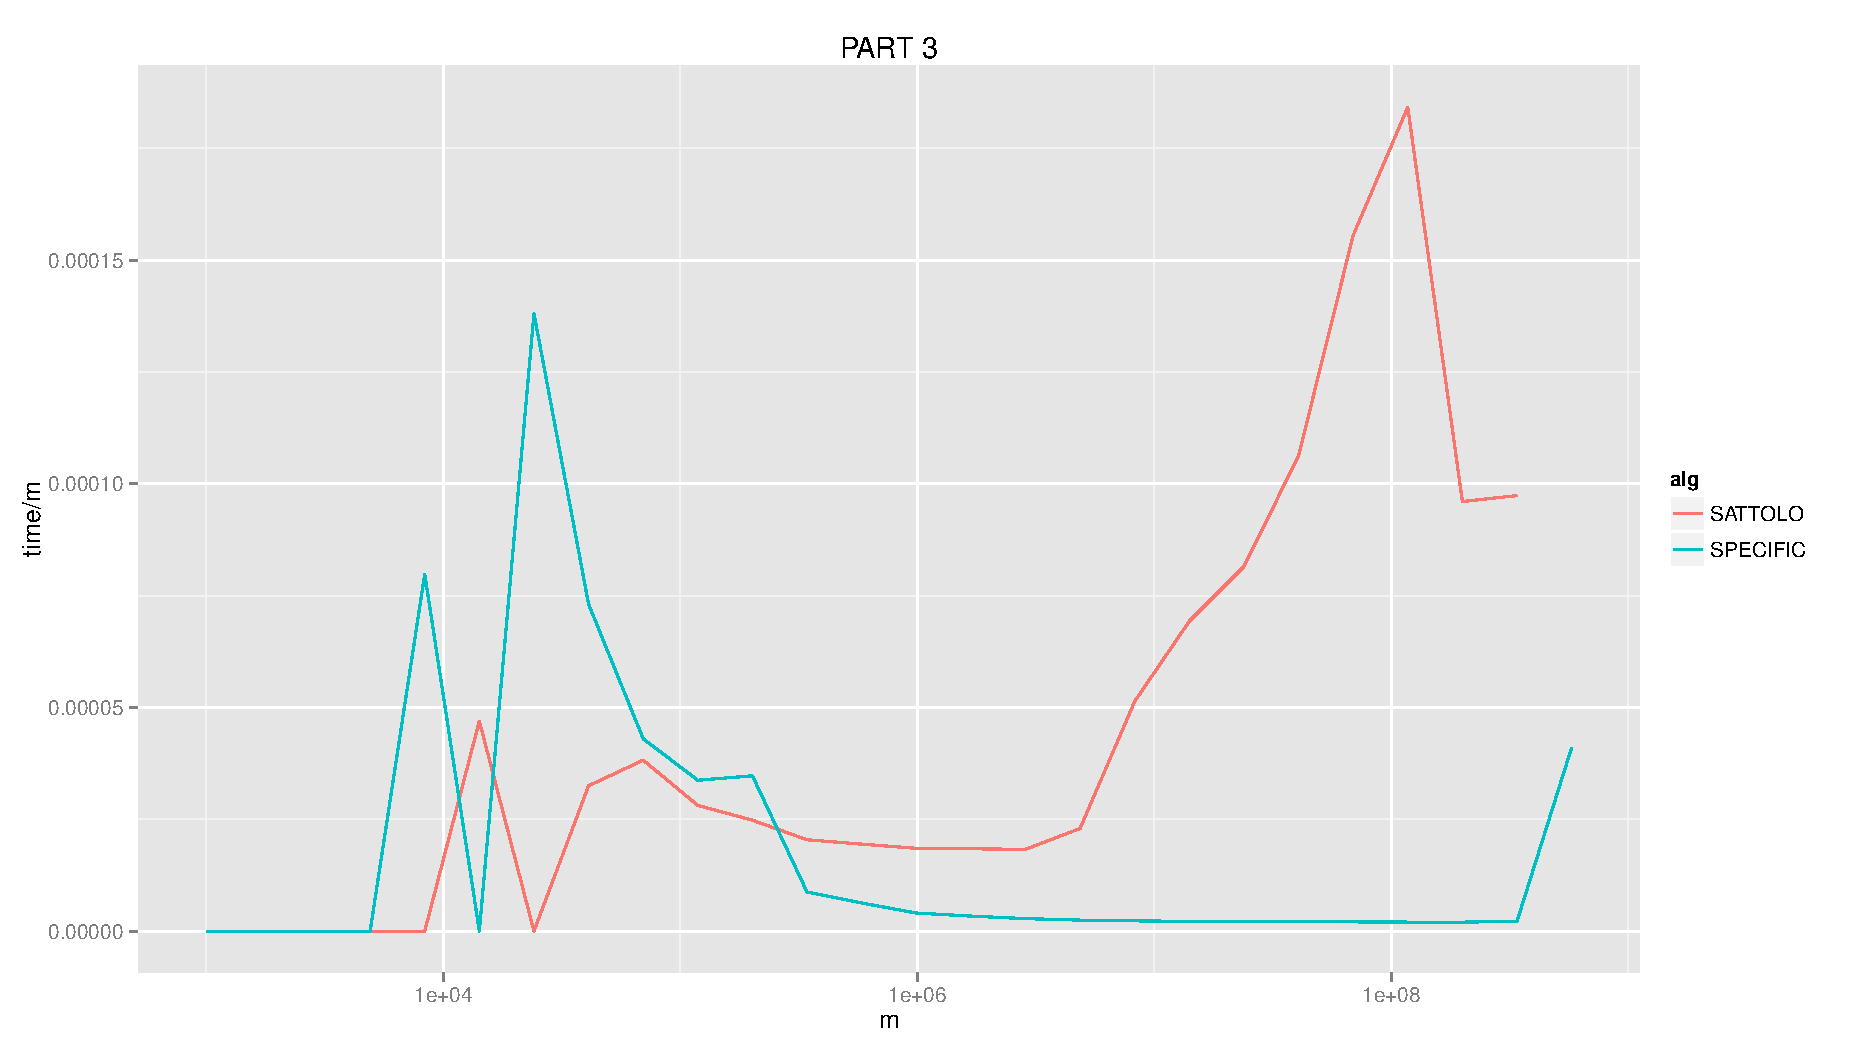
\includegraphics[width=
    \textwidth]{images/part3.pdf}
    \caption{Awesome Image}
    \label{fig:awesome_image}
\end{figure}
\end{document}